\documentclass[11pt]{article}

\usepackage[margin=1in]{geometry}
\usepackage{graphicx}
\usepackage{booktabs}
\usepackage{amsmath}
\usepackage{hyperref}
\usepackage{caption}

\graphicspath{{../figures/}}

\title{From-Scratch Mini LLM: Pre-training and Sentiment Transfer}
\author{Robert Hines}
\date{\today}

\begin{document}

\maketitle

\begin{abstract}
This report describes a compact, from-scratch decoder-only language model
inspired by the Qwen3 family. The model (19.52M parameters) uses Qwen3-family
design choices (RMSNorm, rotary position embeddings, SwiGLU, and grouped-query
capable attention) at a size that trains on CPU; it is not a reproduction of Qwen
at scale. It is pre-trained on the TinyStories corpus with a causal
language-modeling objective and then reused for a binary sentiment task. No
pre-trained weights are used at any stage.
Pre-training reaches a final validation perplexity near 13.9, and the frozen
representations support a sentiment probe at 64.19\% accuracy and 64.03\%
macro-F1, above a 56.00\% majority-class floor. Fine-tuning the base for the same
task raises accuracy to 83.00\%, showing that the representations hold
substantially more sentiment signal than a frozen probe can access. A tokenizer
coverage analysis further shows that although out-of-vocabulary (OOV) rates on
the sentiment domain are high (20.42\%), per-sentence OOV does not predict
misclassification, so adaptation rather than vocabulary coverage is the dominant
lever. The work demonstrates the full path from architectural components to a
working transfer-learning result on commodity CPU hardware.
\end{abstract}

\section{Introduction}
Modern large language models combine a small set of architectural ideas: rotary
position embeddings~\cite{su2021roformer}, RMSNorm~\cite{zhang2019rmsnorm}, and
gated feed-forward layers~\cite{shazeer2020glu}, all built on the transformer
attention mechanism~\cite{vaswani2017attention} and popularized at scale by model
families such as Qwen~\cite{yang2024qwen2}. This project implements those pieces
directly and at a size that trains on CPU, using the TinyStories
dataset~\cite{eldan2023tinystories} for pre-training. The learned representations
are then evaluated on a downstream sentiment task built from an emotion-labeled
sentence corpus~\cite{saravia2018carer}.

\section{Model architecture}
The model is a decoder-only transformer with the following choices:
pre-normalization with RMSNorm, rotary position embeddings applied to queries and
keys, SwiGLU feed-forward blocks, and tied input/output embeddings. Multi-head
attention supports grouped-query attention, though the reported run uses standard
multi-head attention. Table~\ref{tab:arch} lists the configuration.

\begin{table}[h]
\centering
\caption{Model configuration.}
\label{tab:arch}
\begin{tabular}{lr}
\toprule
Hyperparameter & Value \\
\midrule
Parameters & 19{,}520{,}000 \\
Hidden size ($d_{\text{model}}$) & 512 \\
Layers & 6 \\
Attention heads & 8 \\
FFN intermediate size & 1{,}024 \\
Maximum sequence length & 256 \\
Vocabulary size & 7{,}392 \\
Tied embeddings & Yes \\
\bottomrule
\end{tabular}
\end{table}

\section{Data and tokenization}
Pre-training uses the first 10{,}000 TinyStories, split 80/10/10 into training,
validation, and test sets with a fixed seed. A word-level tokenizer is trained on
the training split only, so held-out text does not influence the vocabulary. The
tokenizer keeps four special tokens (padding, beginning of text, end of text, and
unknown) and selects the most frequent remaining tokens, yielding a 7{,}392-token
vocabulary that covers 99.84\% of training-token occurrences. Sequence-length
analysis (Figure~\ref{fig:seqlen}) informed the choice of a 256-token maximum,
which balances coverage against the memory cost of longer contexts on CPU.

\begin{figure}[h]
\centering
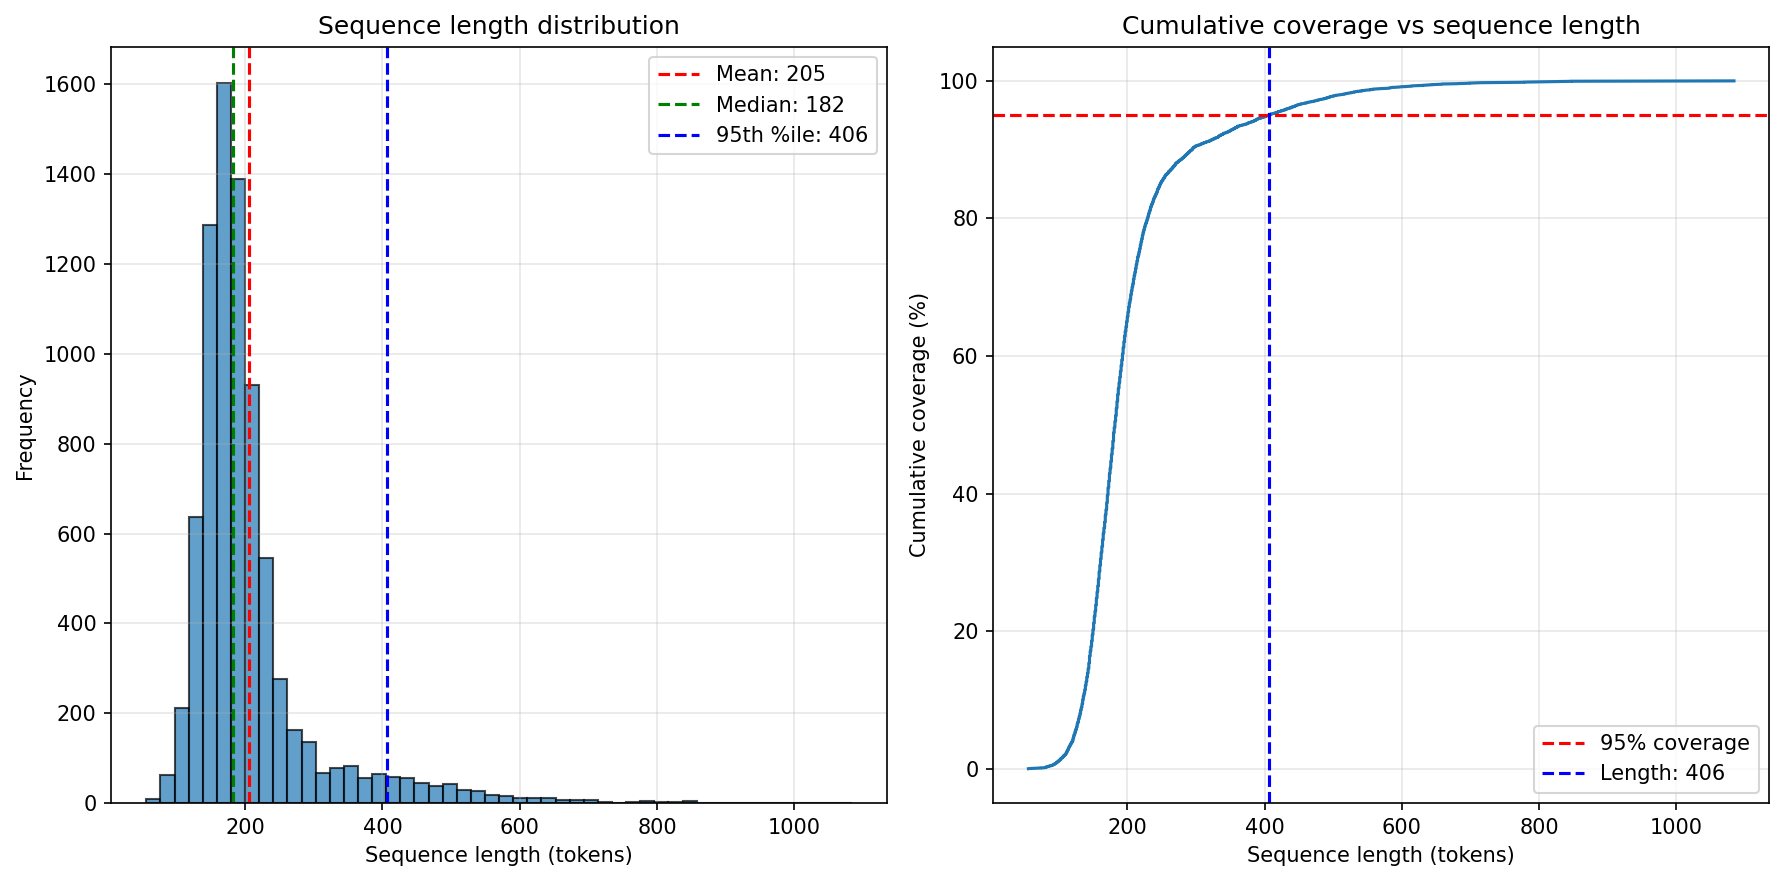
\includegraphics[width=0.95\textwidth]{sequence_length_analysis.png}
\caption{Token-length distribution of the training stories and cumulative
coverage as a function of sequence length.}
\label{fig:seqlen}
\end{figure}

\section{Pre-training}
The model is trained for five epochs (5{,}000 optimizer steps) with a causal
language-modeling loss. Optimization uses AdamW~\cite{loshchilov2019adamw} with
$\beta_2 = 0.95$, which is the Qwen setting and is more stable than the usual
$0.999$ on short sequences, together with gradient clipping and a cosine
learning-rate schedule with linear warmup. Table~\ref{tab:pretrain} summarizes the
outcome, and Figure~\ref{fig:curves} shows the loss and perplexity curves.

\begin{table}[h]
\centering
\caption{Pre-training results.}
\label{tab:pretrain}
\begin{tabular}{lr}
\toprule
Metric & Value \\
\midrule
Total steps & 5{,}000 \\
Final training loss / perplexity & 1.84 / 6.31 \\
Final validation loss / perplexity & 2.63 / 13.90 \\
Best validation loss & 2.61 \\
\bottomrule
\end{tabular}
\end{table}

\begin{figure}[h]
\centering
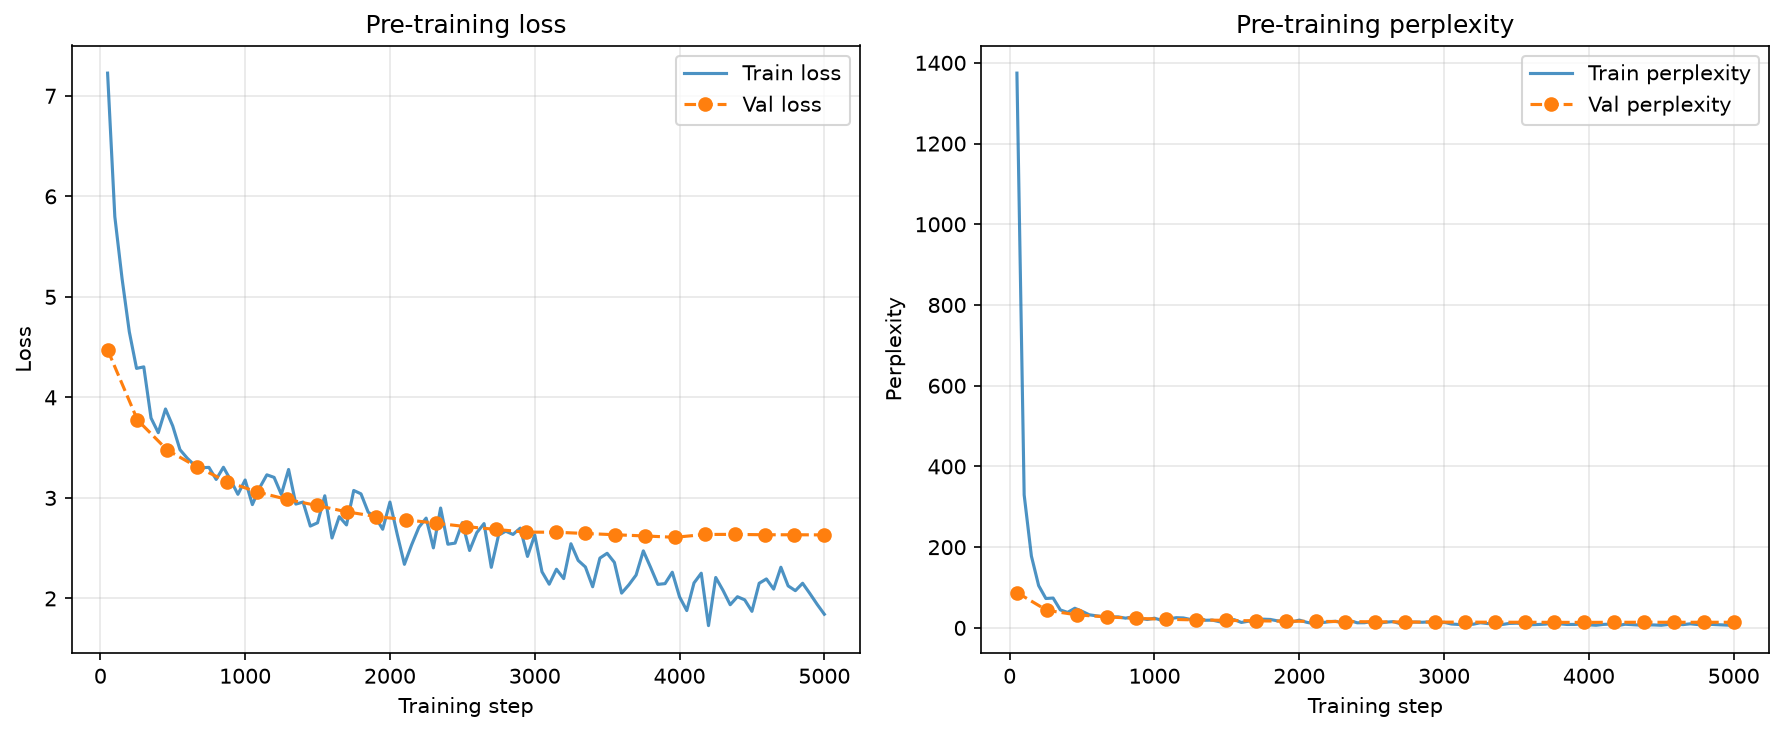
\includegraphics[width=0.95\textwidth]{training_curves.png}
\caption{Pre-training loss (left) and perplexity (right) over training steps, for
both the training batches and periodic validation checkpoints.}
\label{fig:curves}
\end{figure}

\section{Generation}
Text generation supports greedy decoding as well as temperature, top-$k$, and
nucleus (top-$p$) sampling, with optional repetition and no-repeat-$n$-gram
penalties. A key-value cache makes single-prompt generation incremental; rotary
positions are offset by the cached length so a cached decode matches a full
forward pass token for token. At this model scale the samples are coherent within
a few sentences and reflect the simple TinyStories style rather than long-range
narrative structure.

\section{Sentiment transfer}
The downstream task is binary sentiment classification over 16{,}000
emotion-labeled sentences (7{,}238 positive, 8{,}762 negative), split 80/10/10
with the same fixed seed, giving a 1{,}600-sentence test set. The pre-trained
model is frozen and its hidden states are mean-pooled into a single vector per
sentence, which feeds a small MLP head (one 128-unit hidden layer). Only the head
is trained, for 15 epochs at learning rate $10^{-3}$. Freezing the base turns the
task into a probe: it measures how much sentiment signal the language model
captured during pre-training while keeping training inexpensive.
Table~\ref{tab:sentiment} reports test-set metrics with 95\% percentile-bootstrap
confidence intervals (1{,}000 resamples over the fixed test set), and
Figures~\ref{fig:cm} and~\ref{fig:perclass} show the confusion matrix and
per-class breakdown.

\begin{table}[h]
\centering
\caption{Frozen-probe sentiment results (test set). Confidence intervals are 95\%
percentile bootstrap over the test set.}
\label{tab:sentiment}
\begin{tabular}{lrr}
\toprule
Metric & Value & 95\% CI \\
\midrule
Accuracy & 64.19\% & [61.81, 66.63] \\
Macro-F1 & 64.03\% & [61.64, 66.55] \\
Negative precision & 69.96\% & [66.79, 73.12] \\
Negative recall & 63.17\% & [60.02, 66.34] \\
Negative F1 & 66.39\% & [63.84, 68.95] \\
Positive precision & 58.28\% & [54.66, 61.95] \\
Positive recall & 65.48\% & [61.96, 68.91] \\
Positive F1 & 61.67\% & [58.73, 64.78] \\
Best validation macro-F1 & 66.69\% & \\
\bottomrule
\end{tabular}
\end{table}

\begin{figure}[h]
\centering
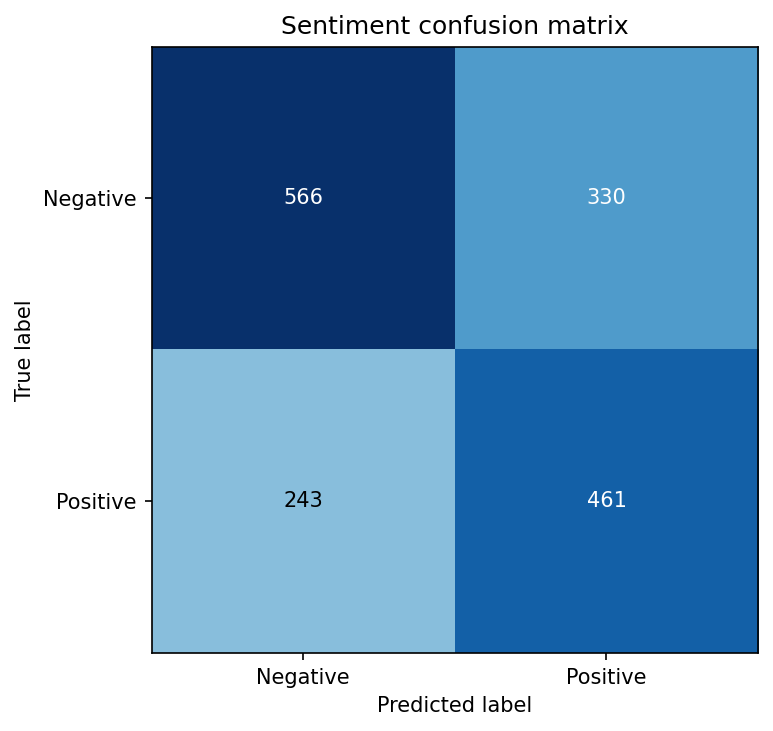
\includegraphics[width=0.55\textwidth]{confusion_matrix_sentiment.png}
\caption{Sentiment confusion matrix on the test set (rows are true labels,
columns are predictions).}
\label{fig:cm}
\end{figure}

\begin{figure}[h]
\centering
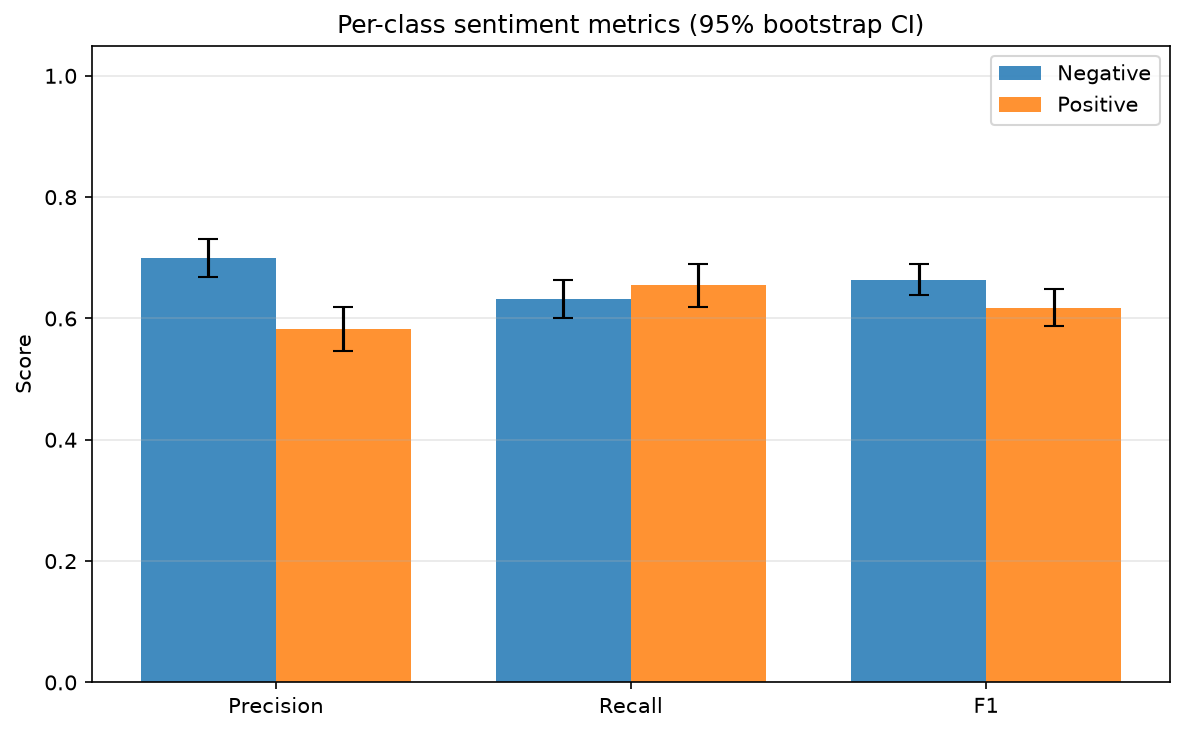
\includegraphics[width=0.75\textwidth]{per_class_metrics.png}
\caption{Per-class precision, recall, and F1 for the frozen probe, with 95\%
bootstrap confidence intervals as error bars.}
\label{fig:perclass}
\end{figure}

\section{Baselines and comparison}
A probe score is only interpretable against reference points. We compare the
frozen probe to a majority-class floor, a lexical baseline (TF-IDF features with
logistic regression), and the identical model with its base fine-tuned rather
than frozen. All four use the same test split. Table~\ref{tab:baselines} and
Figure~\ref{fig:baselines} summarize the comparison.

\begin{table}[h]
\centering
\caption{Sentiment methods on the shared test set.}
\label{tab:baselines}
\begin{tabular}{lrr}
\toprule
Method & Accuracy & Macro-F1 \\
\midrule
Majority class & 56.00\% & 35.90\% \\
Frozen probe (ours) & 64.19\% & 64.03\% \\
Fine-tuned base (ours) & 83.00\% & 82.56\% \\
TF-IDF + logistic regression & 93.19\% & 93.04\% \\
\bottomrule
\end{tabular}
\end{table}

\begin{figure}[h]
\centering
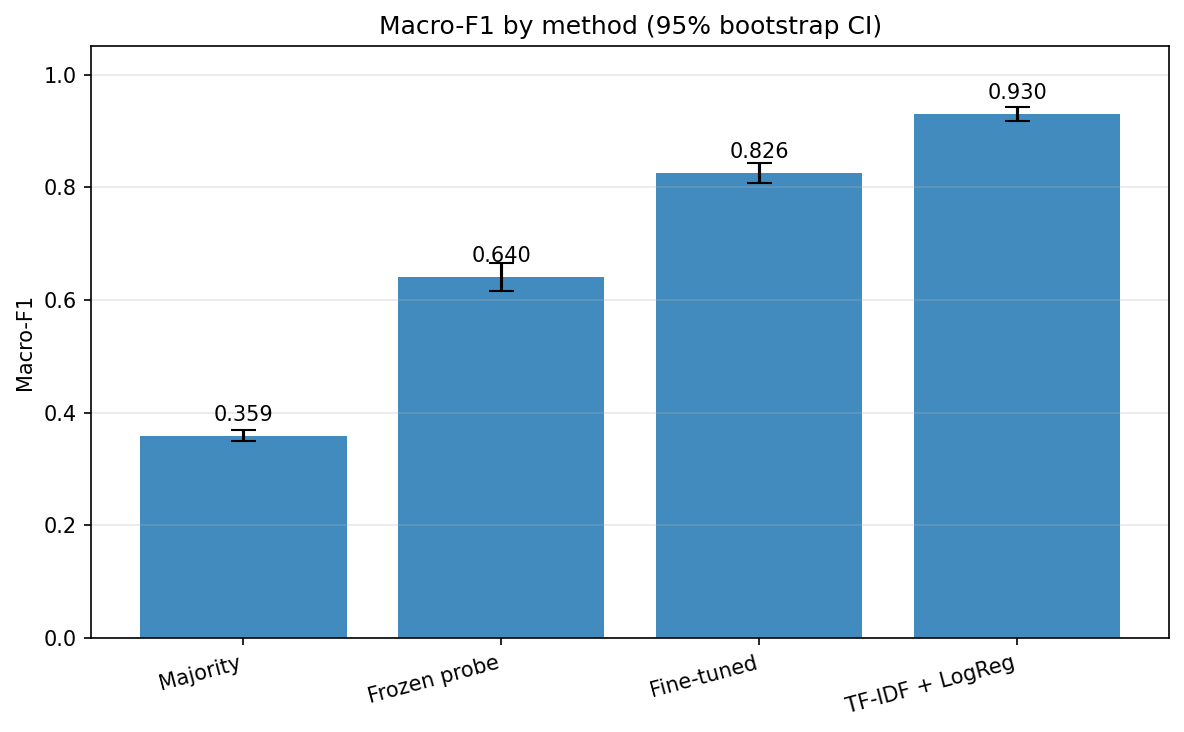
\includegraphics[width=0.85\textwidth]{baseline_comparison.png}
\caption{Macro-F1 by method with 95\% bootstrap confidence intervals. The frozen
probe clears the majority floor with non-overlapping intervals; fine-tuning
closes most of the gap to the lexical baseline.}
\label{fig:baselines}
\end{figure}

The frozen probe clears the majority floor with non-overlapping confidence
intervals, so the pre-trained features carry genuine sentiment signal. Unfreezing
the base lifts accuracy from 64.19\% to 83.00\% (macro-F1 64.03\% to 82.56\%),
recovering most of the distance to the lexical baseline. The frozen probe
therefore understates the information in the representations; adaptation, not
feature quality, is the dominant lever.

\section{Tokenizer coverage and error analysis}
Because the tokenizer was fit on TinyStories, it covers only 79.58\% of sentiment
tokens (20.42\% OOV), and a natural hypothesis is that OOV caps the probe. The
data does not support this at the sentence level. The correlation between a
sentence's OOV rate and being misclassified is $-0.06$; mean OOV is essentially
equal for correct (22.78\%) and incorrect (21.50\%) predictions; and, as
Figure~\ref{fig:oov} shows, accuracy does not decline as OOV rises. OOV is a real
indicator of the domain gap but not the binding constraint here, which is
consistent with fine-tuning rather than vocabulary delivering the large gain.

\begin{figure}[h]
\centering
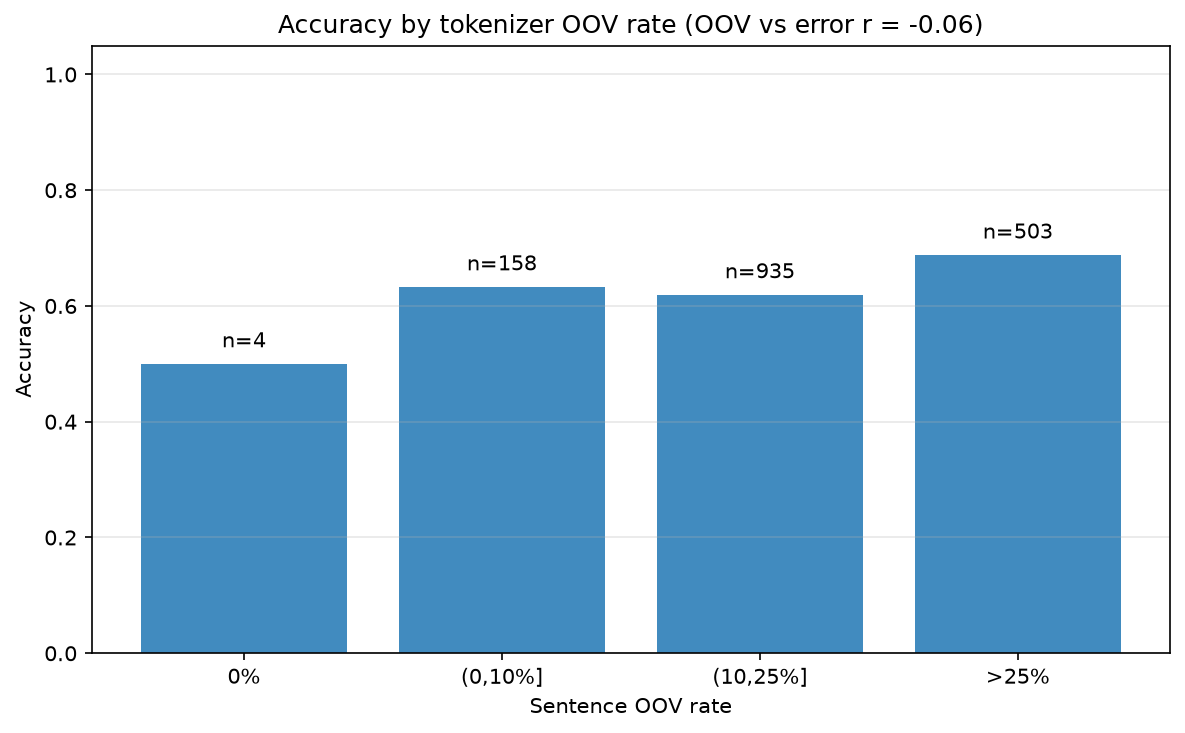
\includegraphics[width=0.85\textwidth]{accuracy_by_oov.png}
\caption{Test accuracy by per-sentence OOV-rate bucket. Accuracy is roughly flat
(and even highest in the largest-OOV bucket), so sentence-level OOV does not
predict error.}
\label{fig:oov}
\end{figure}

\section{Discussion and conclusion}
A 19.52M-parameter model trained on 10{,}000 short stories learns representations
that transfer to sentiment classification well above the majority floor, despite
the large domain gap between children's stories and emotion-labeled sentences.
The frozen probe favors the negative class slightly, consistent with the class
balance in the sentiment data, and lands at 64.19\% accuracy. The more
informative result is comparative: fine-tuning the base reaches 83.00\%, and the
OOV analysis rules out vocabulary coverage as the sentence-level bottleneck, so
representation adaptation is the highest-impact lever. The absolute numbers are
modest but expected given the model size, training budget, and CPU-only setting;
the emphasis here is on a correct, transparent implementation of every stage with
honest baselines and uncertainty rather than on maximizing a benchmark. Natural
extensions include subword tokenization, a larger model and training budget on
GPU, and confidence intervals over repeated training runs to capture seed
variance in addition to test-set sampling.

\begin{thebibliography}{9}
\raggedright

\bibitem{su2021roformer}
J.~Su et al., ``RoFormer: Enhanced Transformer with Rotary Position Embedding,''
\emph{arXiv:2104.09864}, 2021.

\bibitem{zhang2019rmsnorm}
B.~Zhang and R.~Sennrich, ``Root Mean Square Layer Normalization,''
\emph{NeurIPS}, 2019.

\bibitem{shazeer2020glu}
N.~Shazeer, ``GLU Variants Improve Transformer,'' \emph{arXiv:2002.05202}, 2020.

\bibitem{vaswani2017attention}
A.~Vaswani et al., ``Attention Is All You Need,'' \emph{NeurIPS}, 2017.

\bibitem{yang2024qwen2}
A.~Yang et al., ``Qwen2 Technical Report,'' \emph{arXiv:2407.10671}, 2024.

\bibitem{eldan2023tinystories}
R.~Eldan and Y.~Li, ``TinyStories: How Small Can Language Models Be and Still
Speak Coherent English?'' \emph{arXiv:2305.07759}, 2023.

\bibitem{saravia2018carer}
E.~Saravia et al., ``CARER: Contextualized Affect Representations for Emotion
Recognition,'' \emph{EMNLP}, 2018.

\bibitem{loshchilov2019adamw}
I.~Loshchilov and F.~Hutter, ``Decoupled Weight Decay Regularization,''
\emph{ICLR}, 2019.

\end{thebibliography}

\end{document}
